\section{Introduction}
This chapter discloses the results from our study outlined in the previous chapter, building a case for supporting the hypothesis introduced in the previous chapter (Sec. \ref{hypothesis}). We determine the affects of gamification on our system, analysing qualitative user feedback to enrich the findings.
\section{Results of Study Outline}
We analyse the participant's reactions to our system. For some aspects of the study where comparisons are needed, we split the results for user feedback on a  system A/B basis. Unless otherwise specified, results are represented on an emotional scale from 1 -- 5 where `5' represents the most positive response `1' represents the most negative.

The accumulated results can be seen below in Figure \ref{employeeGraph} and \ref{participantGraph}. The participant graph only shows the metrics which were compared between Systems. It is important to highlight that qualitative data is not reflected in these graphs; however the justification of individual replies lie in the qualitative responses --- These will be further discussed in Section \ref{sec:qualitative}.

\begin{table}[h]
\begin{tabular}{@{}ll@{}}
\toprule
\textbf{Question}                                                 & \textbf{Responses}                                \\ \midrule
Does your business have a loyalty scheme?                         & Yes (3/3)                                         \\
What type of loyalty scheme do you run?                           & Stamp Card (2/3) | Reward Card{[}Barcode{]} (1/3) \\
What rewards can the customer claim using the loyalty scheme?     & Free Item (2/3) | Upgrade (2/3)                   \\
What percentage of customers do you feel take part in the scheme? & 40\%-59\% (1/3)|  60\%-79\% (2/3)                 \\ \bottomrule
\end{tabular}
     \caption{A table depicting the different type of loyalty schemes available at the locations the study was run in
     			Chart in Progress IGNORE THE ABOVE GRAPH}
     \label{employeeGraph}
\end{table}


All visited coffee shops the a university campus had at least a paper-based stampcard set in place for a loyalty scheme.  A substantially large percentage of customers seemed to partake in the loyalty scheme (average of 75+\%). One location had a smartcard as well as a paper-stampcard.

%Union loyalty scheme
%Most paperbased etc

\subsection{Participant Questionnaire}
\begin{figure}[H]
 \centering
  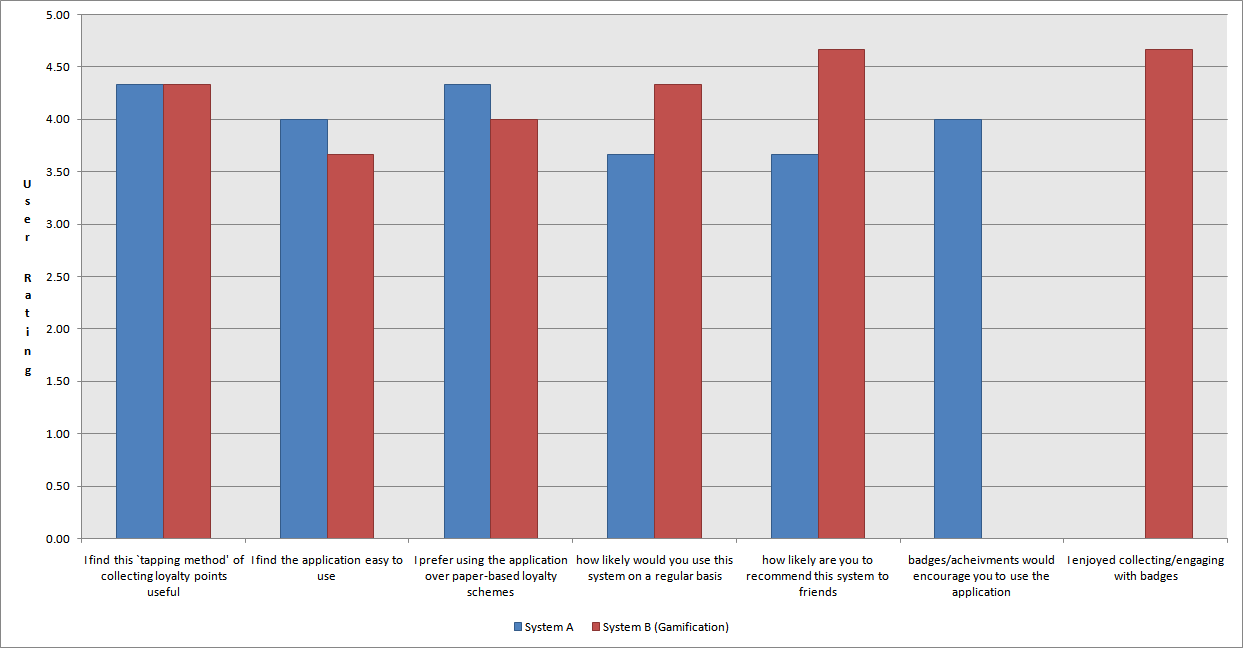
\includegraphics[width=1\textwidth]{img/graph.png}
     \caption{Results of the quantitive questions from the study that compared both systems}
	 \label{participantGraph}
\end{figure}

It is visually evident that questions regarding gamification have a strong positive average response (4+); however there are areas where System A marginally outperforms System B. These areas would be interesting for us to explore further. Both systems appeared to generally receive favourable responses from our participants.
\newpage
\section{Analysis of Questions}
In this section we analyse and discuss each question individually with regards to our hypothesis:
\subsection{Questions 1, 2, 3 --- Participant Loyalty Habits}
With this question we aim to create a portrait of our participant's loyalty habits. We do not use this question to compare our hypothesis as these questions are systems independent--- the aggregated results for these questions are shown below in Table \ref{table:q123}
    \begin{table}[H]
    \resizebox{\textwidth}{!}{%
    \begin{tabular}{@{}llcc@{}}
    \toprule
    \textbf{Question}                                                           & \textbf{Average Response (s.d)} \\ \midrule
    Q1 – Age                                                                    & 21.67 (.577)                              \\
    Q2 - Gender                                                                 & 50\%/50\% Male/Female              \\
    Q3.1 - Stamps Collected Weekly                                              & 3.1 (.633)                             \\
    Q3.2 - I am more likely to complete a stampcard once I start collecting one & 4.0/5.0 (.633)                          \\
    Q3.3 - I occasionally forget/misplace my loyalty cards                      & 3.0/5.0 (1.265)                           \\ \bottomrule
    \end{tabular}
    }
    \caption{Table showing answers to questions 1,2 and 3 from the study}
    \label{table:q123}
    \end{table}
    
As can be seen from the results, the average user collected 3.1 stamps per week; therefore moderate users of loyalty schemes.

There was a wide range of answers regarding forgetting/misplacing loyalty cards but generally there was a disagreement surrounding this question.
        
\subsection{Question 4 --- Technology Acceptance/Ease of Use}
This question models user acceptance of our technology.  Responses are split between systems and can be found in Table \ref{table:q4}
    \begin{table}[H]
    \resizebox{\textwidth}{!}{%
    \begin{tabular}{@{}llcc@{}}
    \toprule
    \textbf{Question}                                                       & \textbf{Average Response (s.d)}                                                                       \\ \midrule
    Q4.1 - I find this `tapping method' of collecting loyalty points useful & \begin{tabular}[c]{@{}l@{}}System A - 4.33/5.0 (.577) \\ System B - 4.33/5 (.577)\\ Total - 4.3/5.0 (.408)\end{tabular} \\ \midrule
    Q4.2 - I find the application easy to use                               & \begin{tabular}[c]{@{}l@{}}\textbf{System A - 4.0/5.0 (.000)}\\ System B - 3.6/5 (.577)\\ Total - 3.8/5.0 (.516)\end{tabular} \\ \bottomrule
    Q4.3 - I prefer using the application over paper-based loyalty schemes & \begin{tabular}[c]{@{}l@{}}\textbf{System A - 4.66/5.0 (.577)}\\ System B - 4.0/5.0 (1.000)\\ Total - 4.33/5.0 (.816)\end{tabular}  \\ \midrule
    \end{tabular}
    }
    \caption{Table showing answers to question 4 from the study}
    \label{table:q4}
    \end{table}
    
    Participants agreed on the usefulness of the tapping method to collect stamp.
    
    Participants with System B found the system harder to use than those using System A.

	There are several explanations why addition of gamification seemed to make the application more difficult to use. Badges may have been implemented in such a way that clutters the interface, making it harder to user. On the other hand, by referencing the Technology Acceptance Model (Fig. \ref{fig:TAMagain}), the `easy to use' metric does not impact acceptance factors very much, they only affect the attitude towards using the system.  It is the `perceived usefulness' of the application that can directly affect the attitude and behavioural intention to use the system.
    \begin{figure}[H]
 \centering
  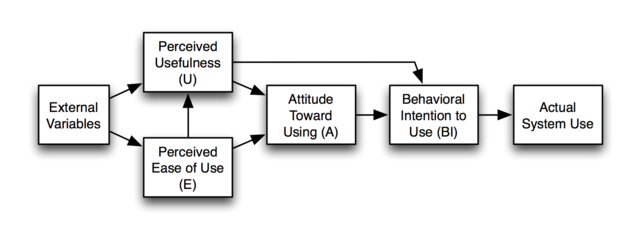
\includegraphics[width=0.80\textwidth]{img/TAM.png}
     \caption{The Technology Acceptance Model (TAM) displaying that `Perceived easy to use' has far more impact on behaviour to use than `easy to use'}
     \label{fig:TAMagain}
\end{figure}
    
\subsection{Question 5 --- User Enjoyment/Recommendation}
This metric is one which we use to gauge user enjoyment of the system. Individuals who enjoy the system and find it easy to use are more likely to use it themselves and recommend it to others. The feedback can be found in Table \ref{table:q5}.
    \begin{table}[H]
    \resizebox{\textwidth}{!}{%
    \begin{tabular}{@{}llcc@{}}
    \toprule
    \textbf{Question}                                                      & \textbf{Average Response (s.d)}                                                                            \\ \midrule
    Q5.1 - How likely would you use this system on a regular basis         & \begin{tabular}[c]{@{}l@{}}System A - 3.66/5.0 (1.154)\\ \textbf{System B - 4.33/5.0 (1.154)}\\ Total - 4.0/5.0 (1.094)\end{tabular}  \\ \midrule
    Q5.2 - How likely are you to recommend this system to friends          & \begin{tabular}[c]{@{}l@{}}System A - 3.66/5.0 (1.154)\\ \textbf{System B - 4.66/5.0 (.577)}\\ Total - 4.17/5.0 (.983)\end{tabular} \\ \bottomrule
    \end{tabular}
    }
    \caption{Table showing answers to question 5 from the study}
    \label{table:q5}
    \end{table}
    \newpage
   	Participants using System B were more likely to use the system on a regular basis and recommend Stamped to friends than those testing System A. 
   	
	\textbf{Q5.1 Hypothesis supported}

	\textbf{Q5.2 Hypothesis supported }   
    
\subsection{Question 6 \& 7 --- Gamification In The System}
Question 6 was exclusive to those that tested System A (without gamification), whereas question 7 was exclusive to System B (with gamification). The purpose of question is to get explicit feedback regarding badges and titles --- results are shown below in Table \ref{table:q67}. 
    \begin{table}[H]
    \resizebox{\textwidth}{!}{%
    \begin{tabular}{@{}llcc@{}}
    \toprule
    \textbf{Question}                                                  & \textbf{Average Response (s.d)} \\ \midrule
    Q6 - Badges/achievements would encourage you to use the application        & System A - 4.17/5.0 (1.000)                  \\ \midrule
    Q7 - I enjoyed collecting/engaging with badges					  & System B - 4.66/5.0 (0.588)                  \\ \bottomrule
    \end{tabular}
    }
    \caption{Table showing answers to questions 6 and 7 from the study}
    \label{table:q67}
    \end{table}
    
    Question 6 asked participants using System A how much value they would perceive badges/achievements would add to the system.
    
    Question 7 explicitly asked participants if they enjoyed the gamification elements included in the application and whether they gained value in engaging with them. 
    
    In both systems, responses were far more positive in System B than System A:    

    \textbf{Q6 - Hypothesis supported}
    
    \textbf{Q7 - Hypothesis supported}

\section{Analysis of Qualitative Feedback}
\label{sec:qualitative}
Here we analyse qualitative feedback that was gathered from both the questionnaire and general responses
\subsection{Researcher Observations}
Accompanying the participant responses, the researcher aggregated some findings from observing the participants over the study --- these are discussed below.
\subsubsection{Predictability of the Interaction}
As earlier identified in chapter 6, `weak NFC interactions` were issues caused by several factors, we attempted in the actual study to mitigate their occurance by changing the way we instruct paricipants to tap the reader. Nonetheless, at every meeting at least one weak interaction occurred with participants. Though this is a high-priority issue that needs resolving in the future, we predict that implementing the ideal solution \ref{XXXXX}, would greatly reduce the rates of weak interactions.
\subsubsection{Keeping the Application Open To Stamp}
Although Host Card Emulation does allow users to collect stamps without having the application open, almost all participants chose to have the application open when tapping the reader. When questioning one participant on the matter, they suggested that they trusted that the interaction would complete more reliably if they had Stamped open. This is primarily due to Host Card Emulation running in the background on the device, therefore hinting making it difficult for users to tell if the service is running when the application is not open.

One participant mentioned that he wanted to tap the reader without having the screen on/application open. Unfortunately in the interests of battery life, this is not a possible or preferable solution. 
\subsection{Gamification Feedback}
The general response towards gamifcation was strongly positive. Several individuals suggested adding more meaning to the badges as they seemed to mainly serve aesthetic purposes; nonetheless Sociality (Sec. \ref{sec:invite}) was a discussed as a potential solution.

Asking participants that tested System A their opinion about adding badges proved to be very interesting. As System A participants never get to see the system with gamification, their perception would be of `their ideal implementation' instead of our own. More specifically, if they cannot imagine the value gamification adds to their system in their imaginary implementation, then it may not be useful to have at all.

One individual (tested System A) highlighted that the gamification would be redundant as a motivator. When questioned why, they said that there already exists motivations to use the system in order to reap the rewards of loyalty schemes; therefore the addition of gamification would seem to be `bolted on'. This is a valid criticsm of our implementation as there is no direct link between gamification and the loyalty schemes themselves. We can remediate this in several ways, firstly by allowing the creation of more complex badges (i.e. Visit all loyalty schemes in an area) and secondly, deeply integrating gamification principles to the rewards themselves; for instance a solution similar to Starbucks' method of levelling up loyalty schemes.

\section{Limitations of Study}
This section outlines several factors which limited our study or analysis as a result.

The amount of participants perhaps could have been increased; however a key requirement of participants for our study was an Android phone of a compatible version to run by stamped. Moreover running field study sessions with all participants present would become a logistically strenuous task. One solution to counteract this would be to test the system in a different context (i.e. Gym passes, Bike Miles etc).
   
Only a single type of gamification was tested for our A/B testing, meaning that our results may not suggest positive response to gamification as a whole but only to our specific implementation of badges.  A different way to run the study would be to have three control groups, System A with no gamification, System B with Badges and System C with a different type of gamification. This would allow us to get a more holistic feedback on gamification in our system, as well as the gamification technique users prefer. 

In terms of analysing user reactions to gamification, it can be difficult to ask users how they feel about adding badges into the system if they tested the system without them. On the other head, this questions users regarding whether they would see value in its implementation. %idealistic

\section{Feedback on the Final Designs}
Throughout the process of design to the evaluation, feedback was gathered on the final design of the Stamped (Fig. \ref{fig:wireframer3}) and Stamped Manager (Fig. \ref{fig:wireframemr2}). In the interests of time, we will not perform any further iterations on the system design; however this feedback will be vital for future work.
\subsection{Stamped}
\begin{figure}[H]
 \centering
  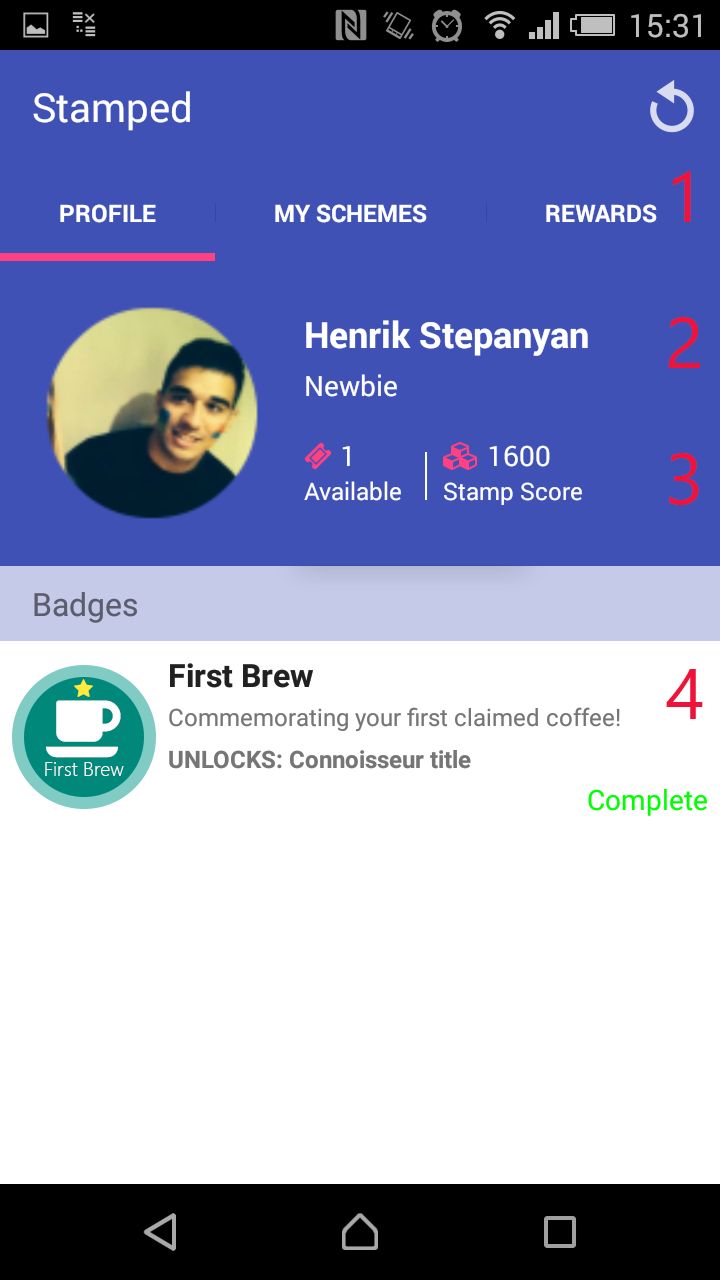
\includegraphics[width=0.275\textwidth]{img/moremock2.png}
   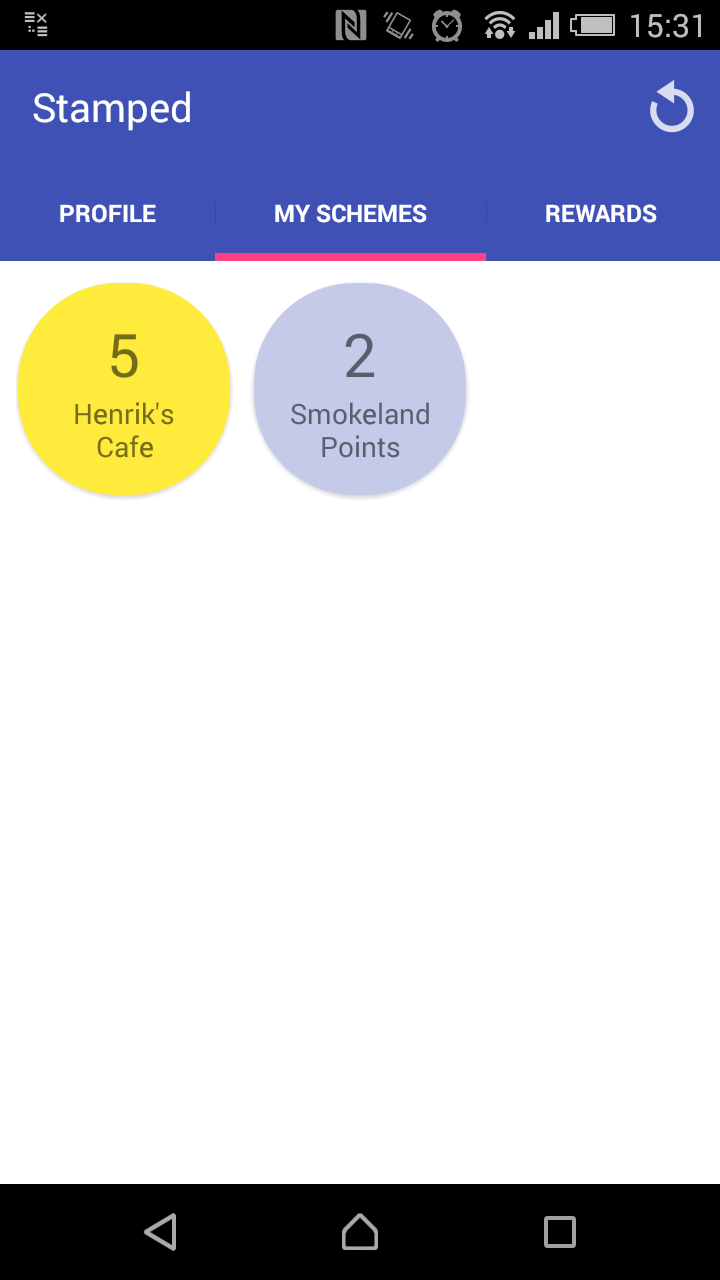
\includegraphics[width=0.275\textwidth]{img/finalmock.png}
    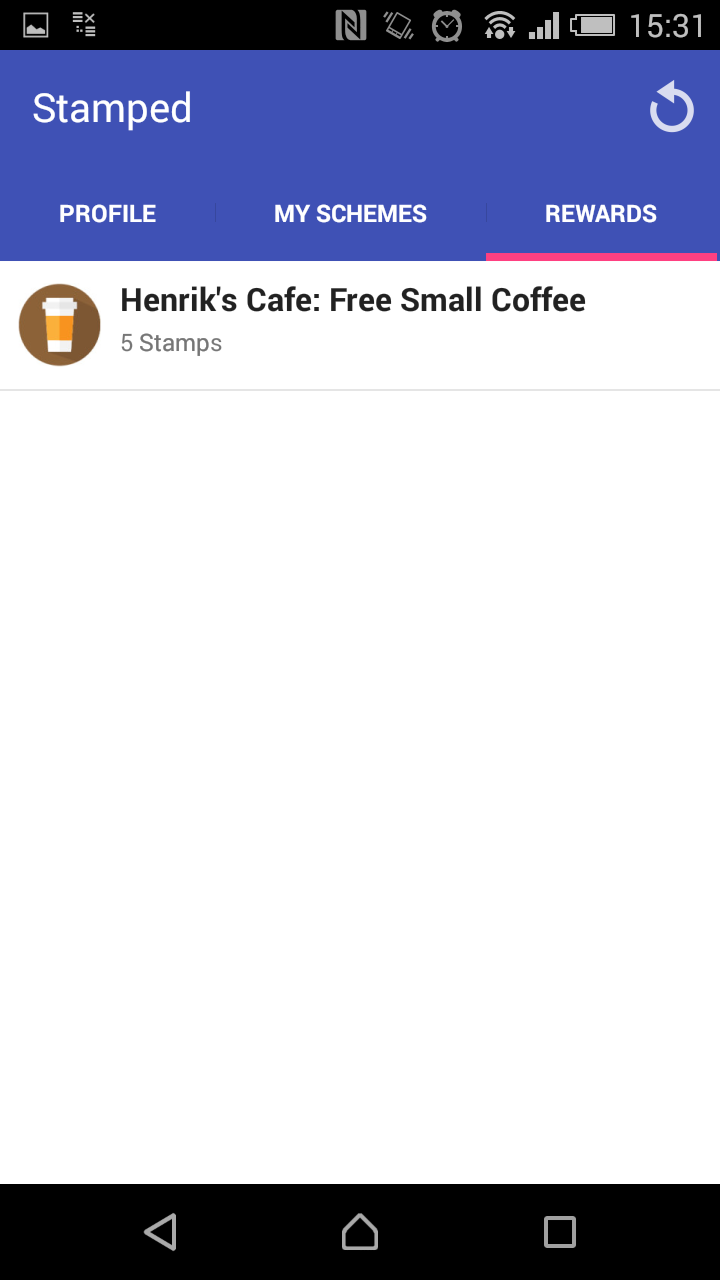
\includegraphics[width=0.275\textwidth]{img/moremock1.png}
     \caption{The final design of Stamped with a tabbed interface}
     \label{fig:wireframer3}
\end{figure}

\subsubsection{Feedback For Next Iteration}
The design was present to three potential users individually, along with all participants during the evaluation, a list of their suggestions follows:
\begin{itemize}
  \item \textit{``There should be more room for businesses to customise their schemes according to their brand''}
  \item \textit{``Single rewards per loyalty scheme is great, but the design doesn't accommodate multiple rewards very well''}
  \item \textit{``There should be more clarity in the app when I get a stamp (e.g. red badge over My Schemes)''}
\end{itemize}

\subsection{Stamped Manager}
\begin{figure}[H]
 \centering
  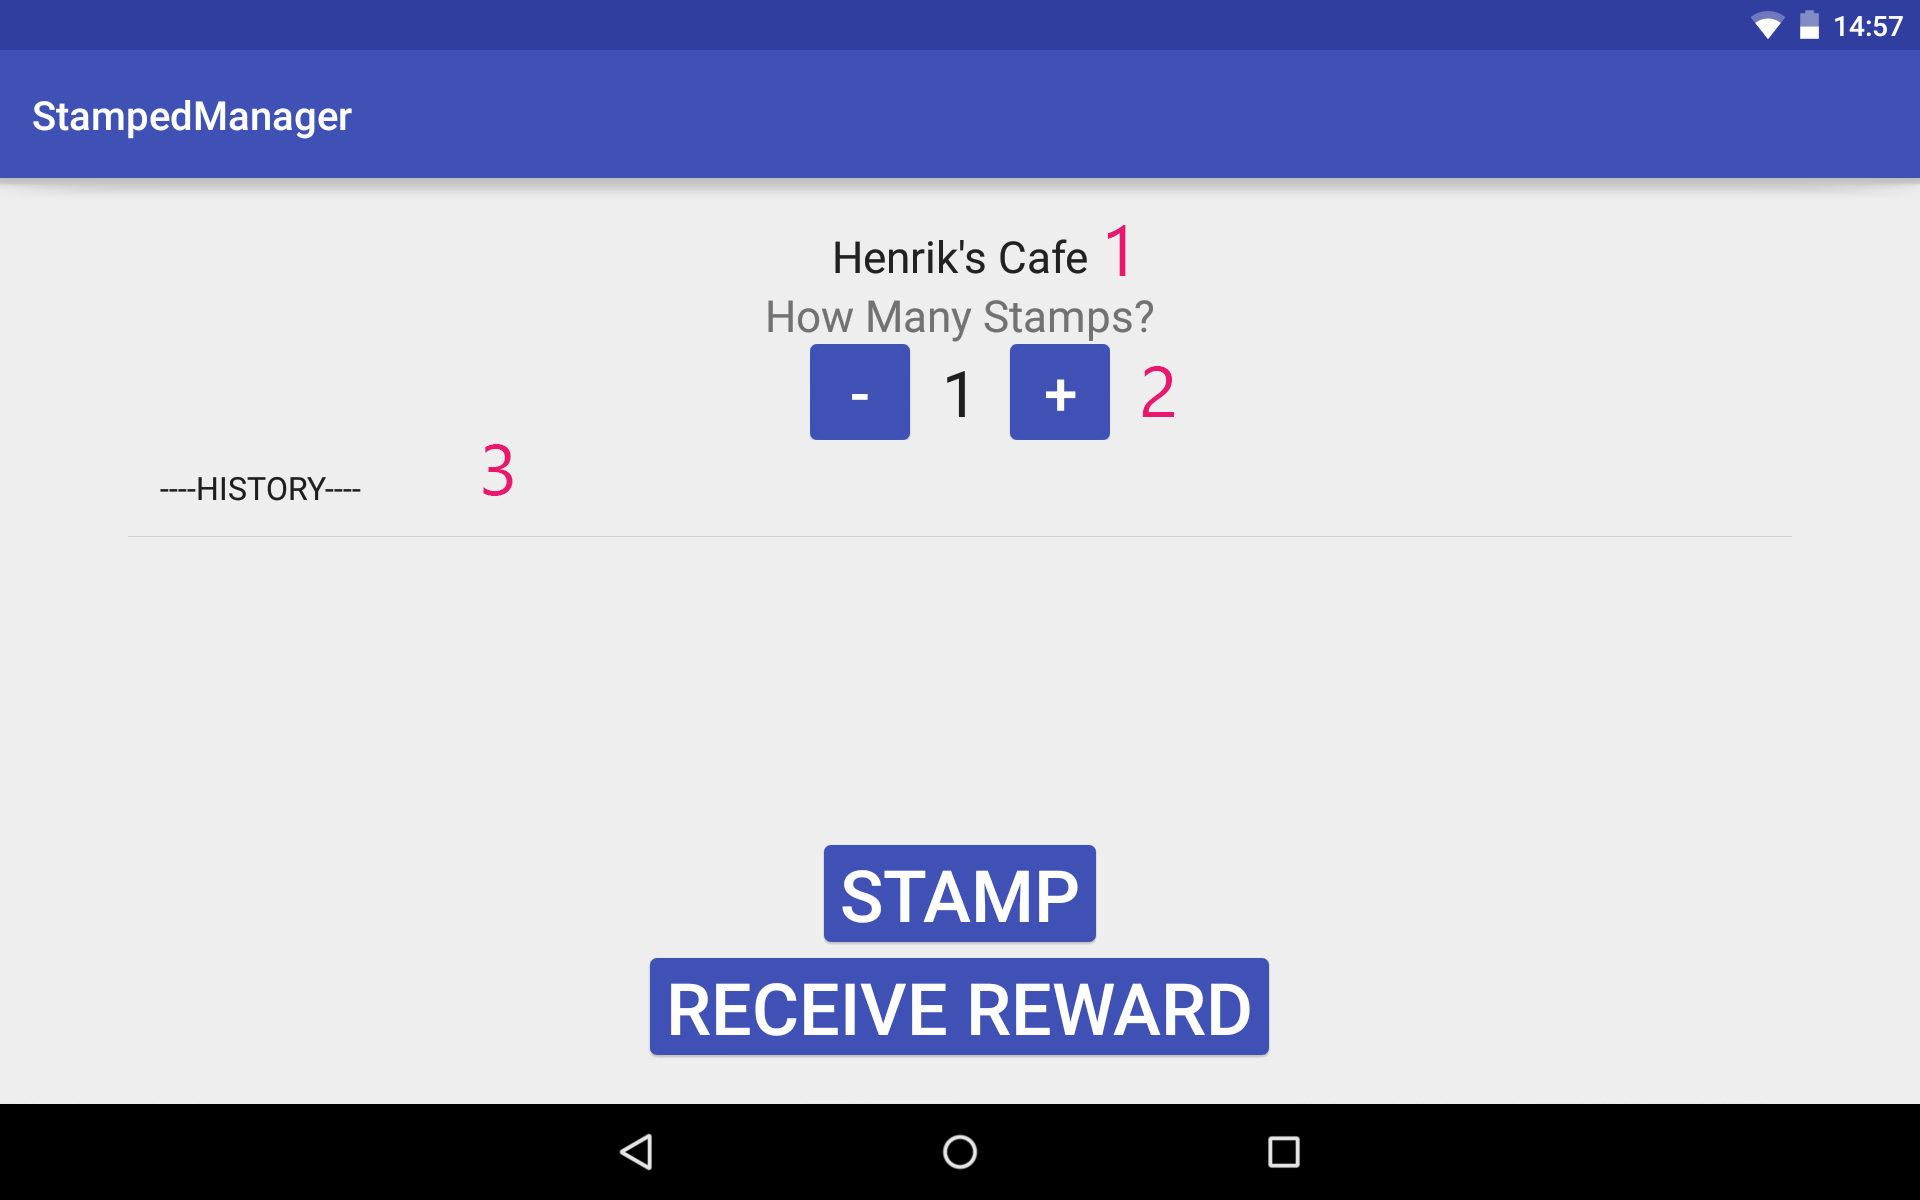
\includegraphics[width=0.494\textwidth]{img/readerfinalmock2.png}
   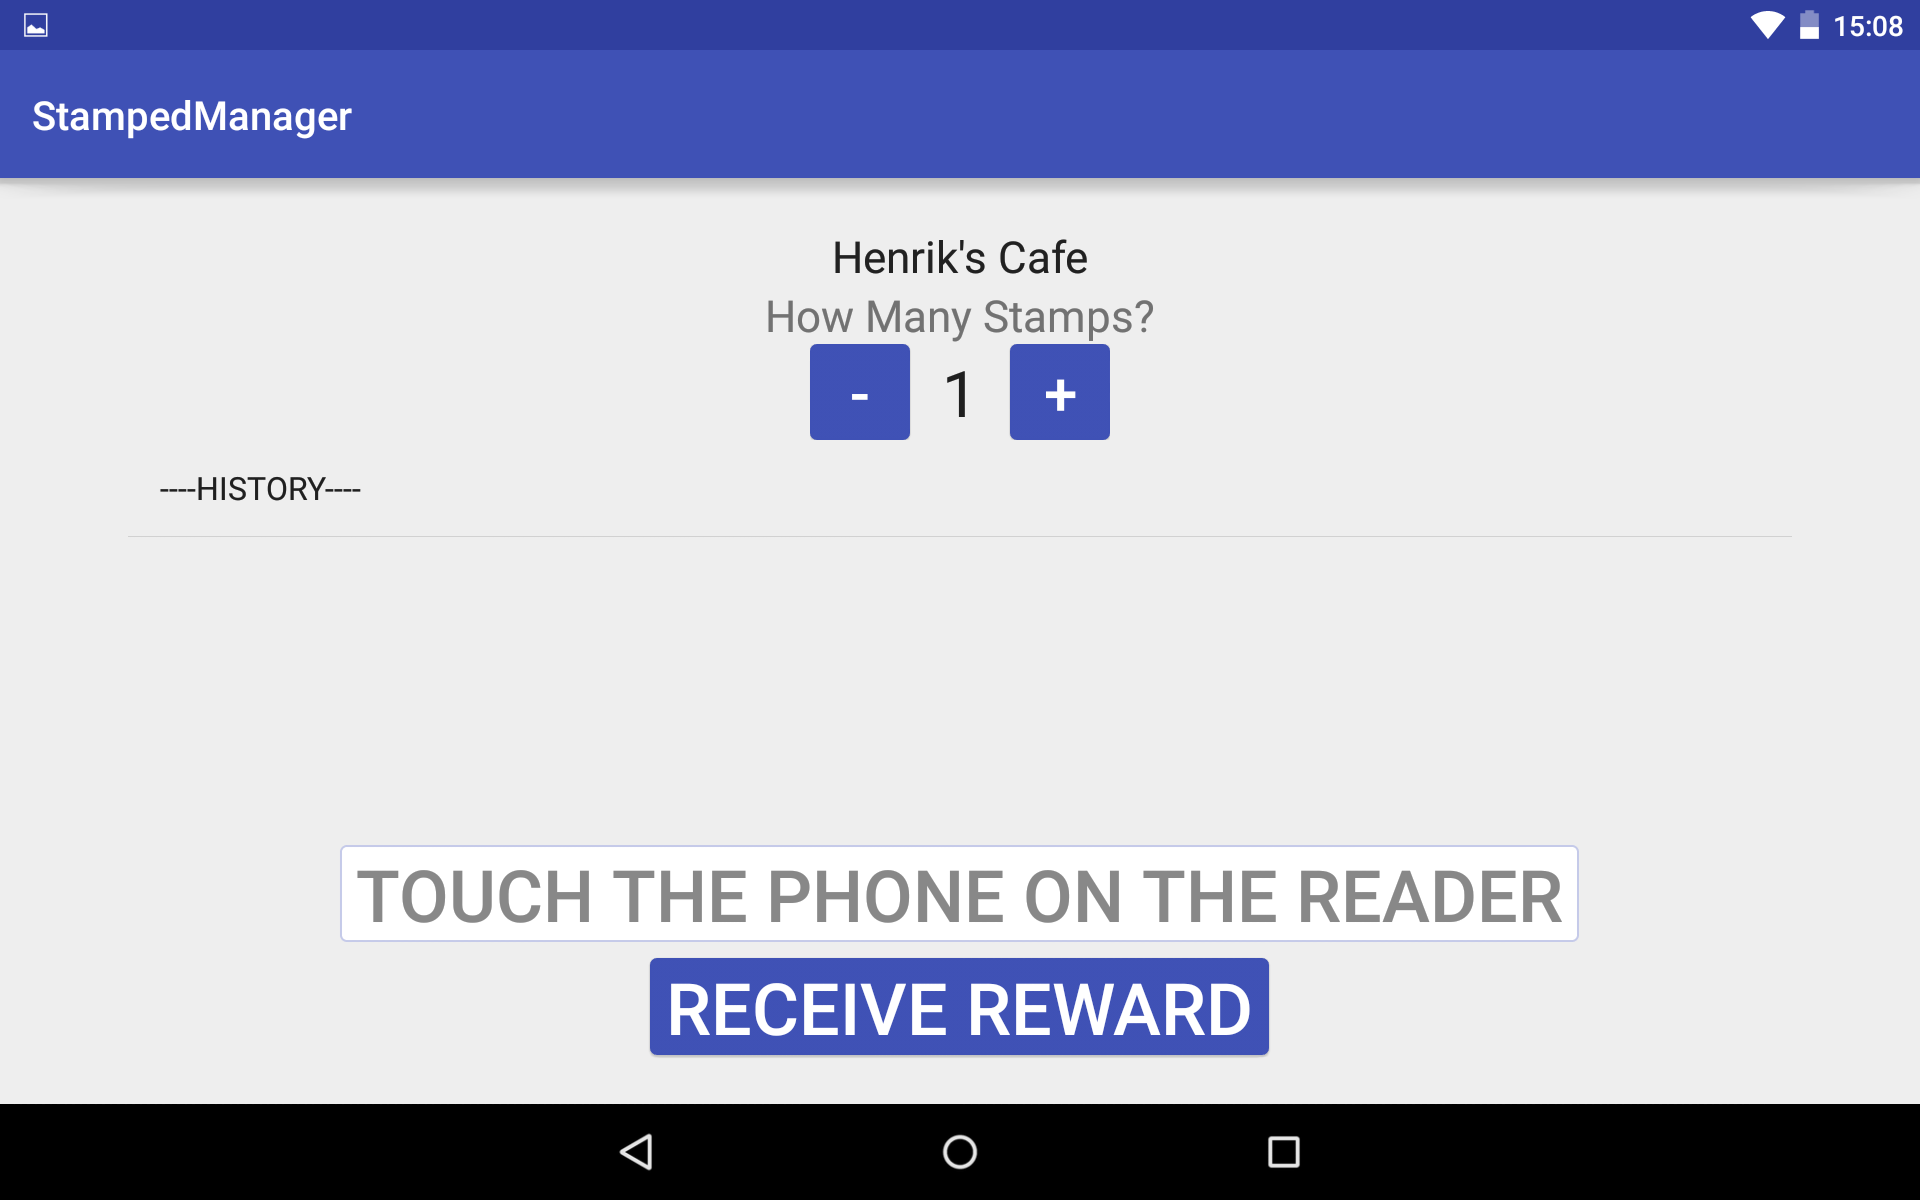
\includegraphics[width=0.494\textwidth]{img/readerfinalmock1.png}
     \caption{The final design of the Stamped Manager with the final aesthetic}
     \label{fig:wireframemr2}
\end{figure}

\subsubsection{Feedback For Next Iteration}
The design was present to three potential users individually, along with all participants during the evaluation, a list of their suggestions follows:
\begin{itemize}
  \item \textit{``The buttons could be bigger like the original design''}
  \item \textit{``There should exist an option to go back to the select a scheme page''}
  \item \textit{``Transaction history need a way to be backed up''}
  %Transaction history PII
\end{itemize}

\section{Miscellaneous Feedback}
\subsection{Customisability}
Participants expressed a keen interest improving the customisability of their profile. Although badges, and titles received a positive response, by increasing user customisation, users will be more inclined to spent time in creating their profile; therefore encouraging their investment to the system.~\cite{winWithGamification}. Another type of customisation would be to allow users to have more control over their schemes (i.e. arrange them by preference, sort by proximity to businesses, delete unused schemes etc).
\subsection{Invite Friends/Get Rewards}
\label{sec:invite}
One participant recommended the ability to invite friends as a means get rewards/grow the Stamped ecosystem. In fact, many gamified systems have a social element. There are two possible reasons for this, to be able to show off earned status (leaderboards, badges) to friends and to pander to the viral coefficient~\cite{viral}. The viral coefficient represents the spread of a system/campaign through referrals by current adopters. A high steady coefficient models the growth of a userbase.%viral coefficient////show off
\subsection{Out of Box Experience}
The application was missing substantial instructions on how to operate the system, that were instead outlined in the brief and instructions to the participants. We discussed in chapter 2 the notion of tools in Foggs taxonomy as a method of helping users reach specific goals. Many mobile applications have Out-Of-Box-Experiences (OOBEs) (Fig. \ref{fig:OOBE}). These are one-time screens presented to the user when they first install a mobile application,  serving as a tool with the goal of instructing the user on key functionality to get started. 
\begin{figure}[H]
 \centering
  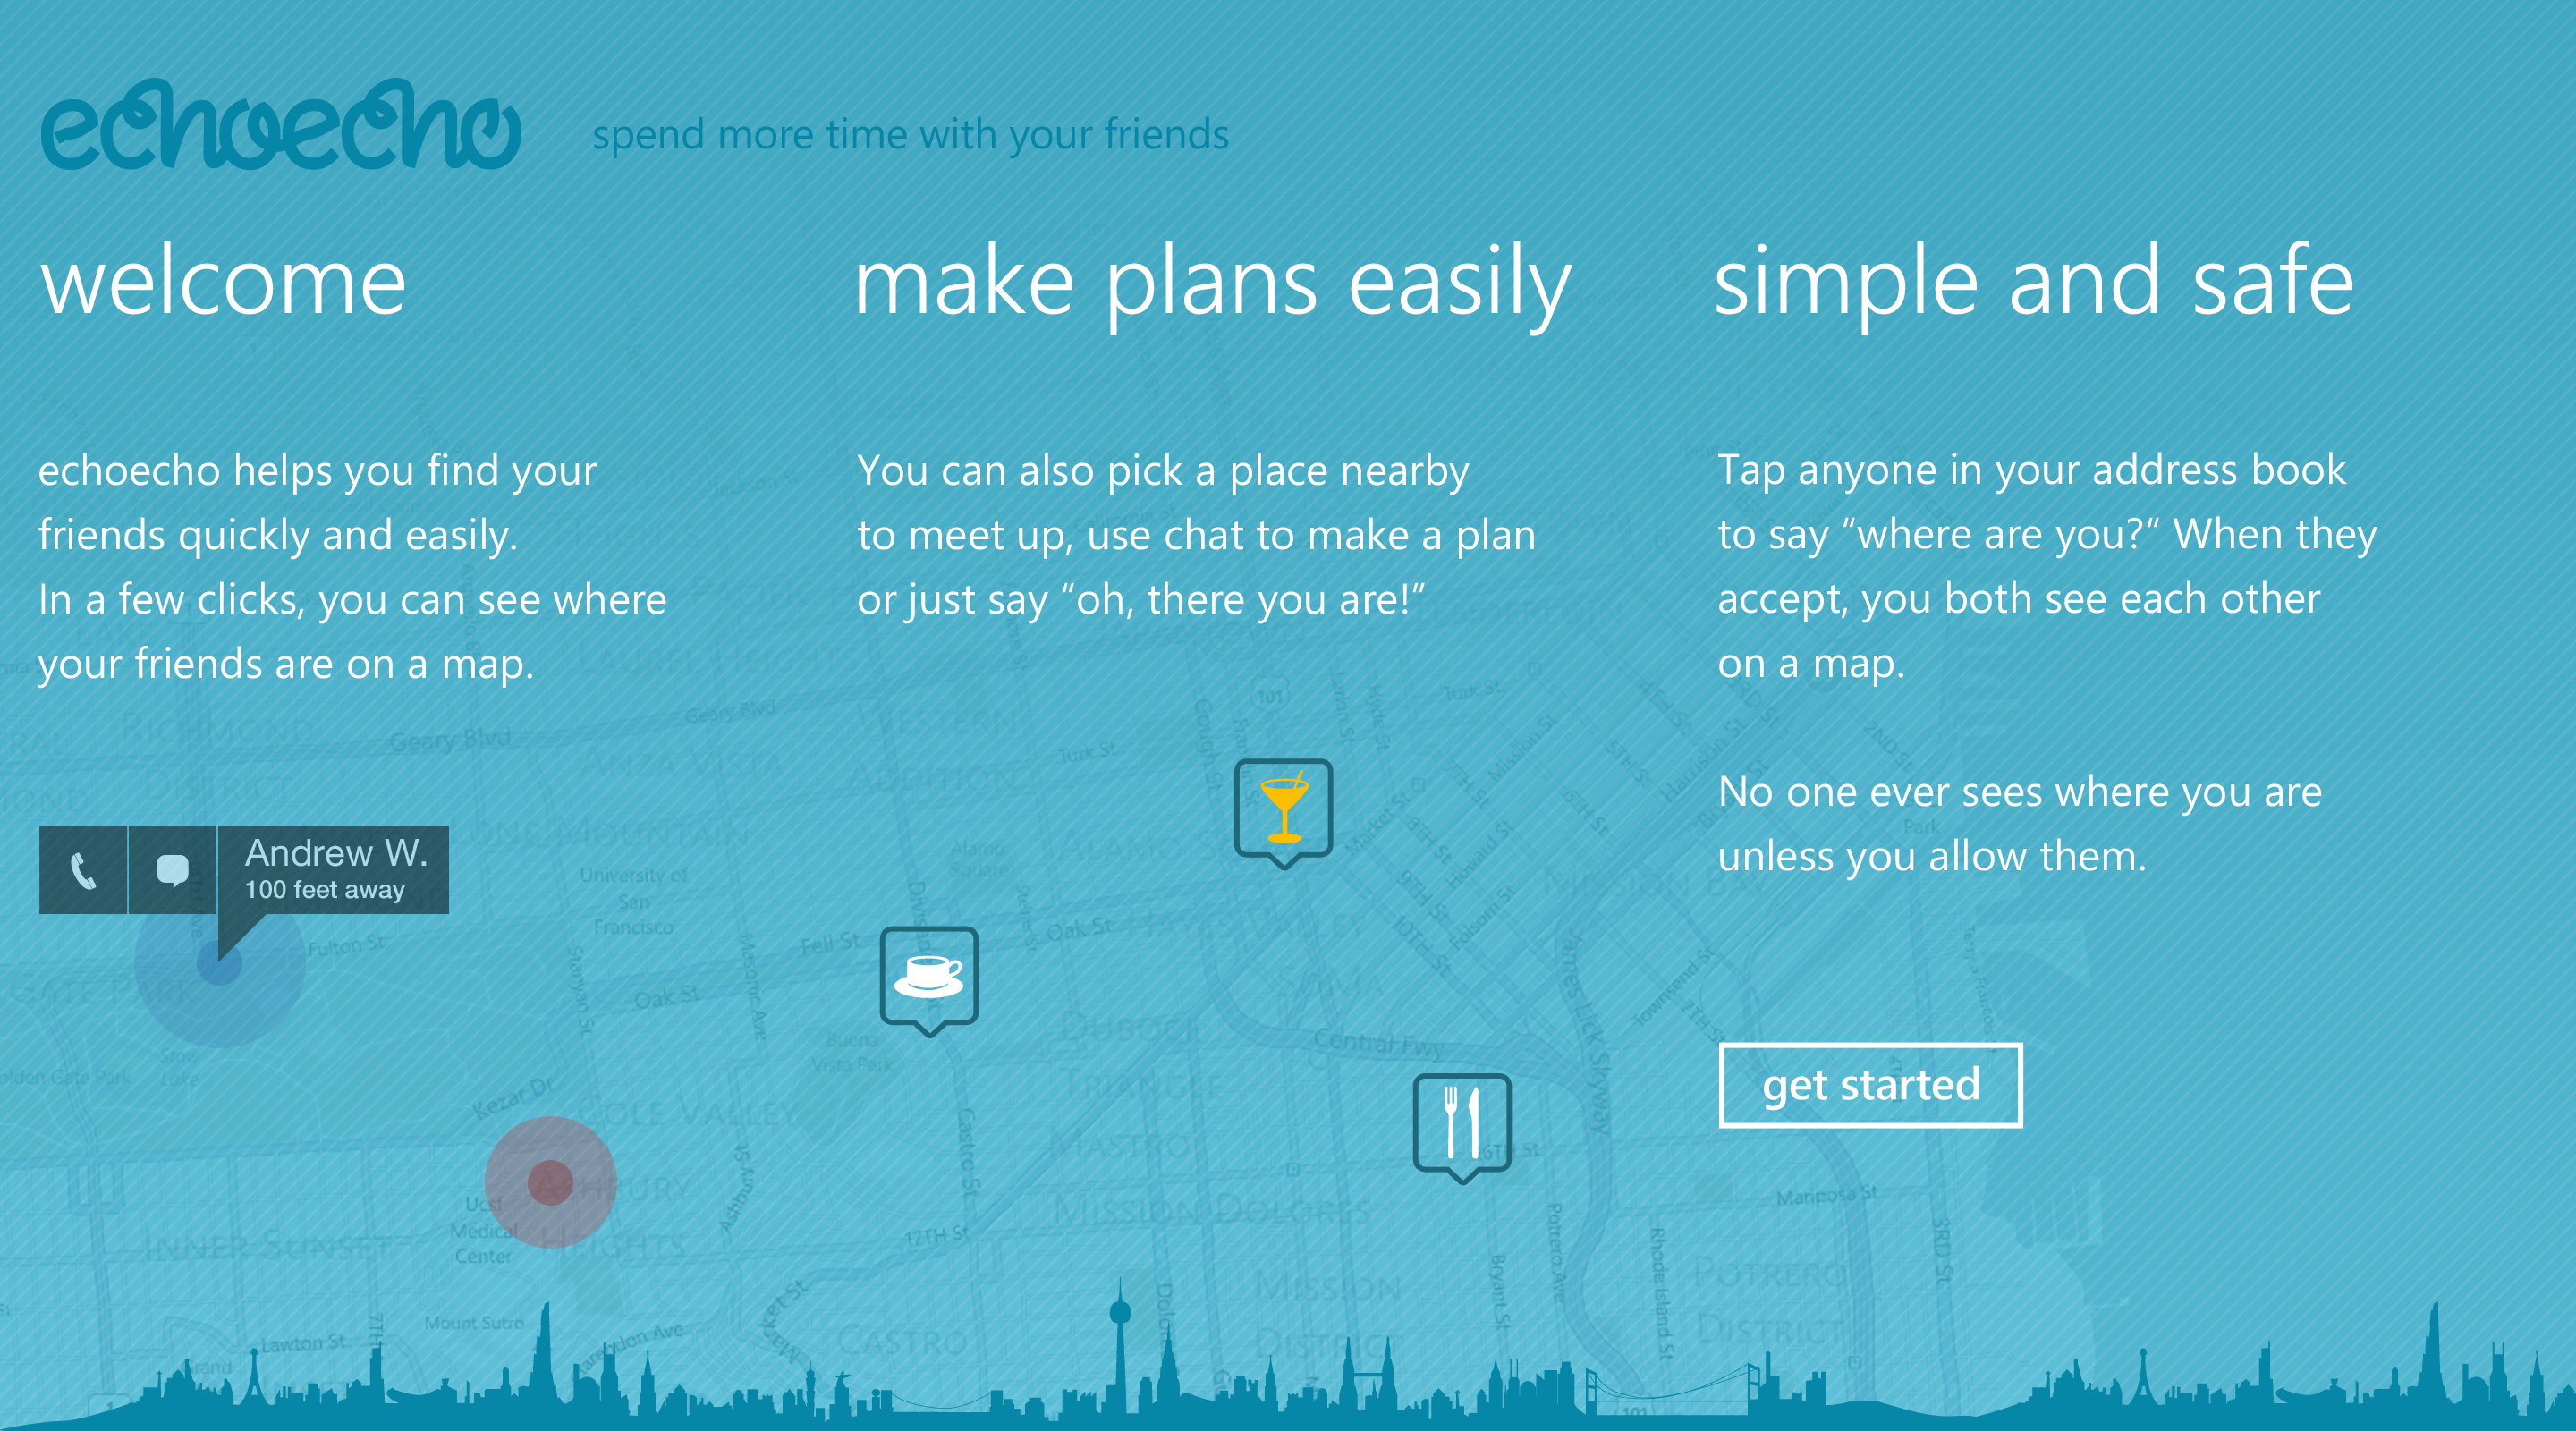
\includegraphics[width=0.6\textwidth]{img/OOBE.png}
     \caption{A panorama of the OOBE found in the \emph{echoecho} application}
     \label{fig:OOBE}
\end{figure}
\section{Conclusion}
In this chapter we looked at the results of our study and the impact gamification has had on the system. We conclude that gamification did indeed bring value to Stamped, 

In the next chapter, we summarise our project in terms of its process, contribution to the state of art and ideas for future work. 